\subsection{Langkah Praktikum: A* untuk Pencarian Rute Terpendek}
Praktikum 9 menerapkan A* pada graf berbobot. Graf disimpan sebagai adjacency list, sedangkan heuristik dihitung dari jumlah busur minimum menuju target.

\begin{figure}[H]
    \centering
    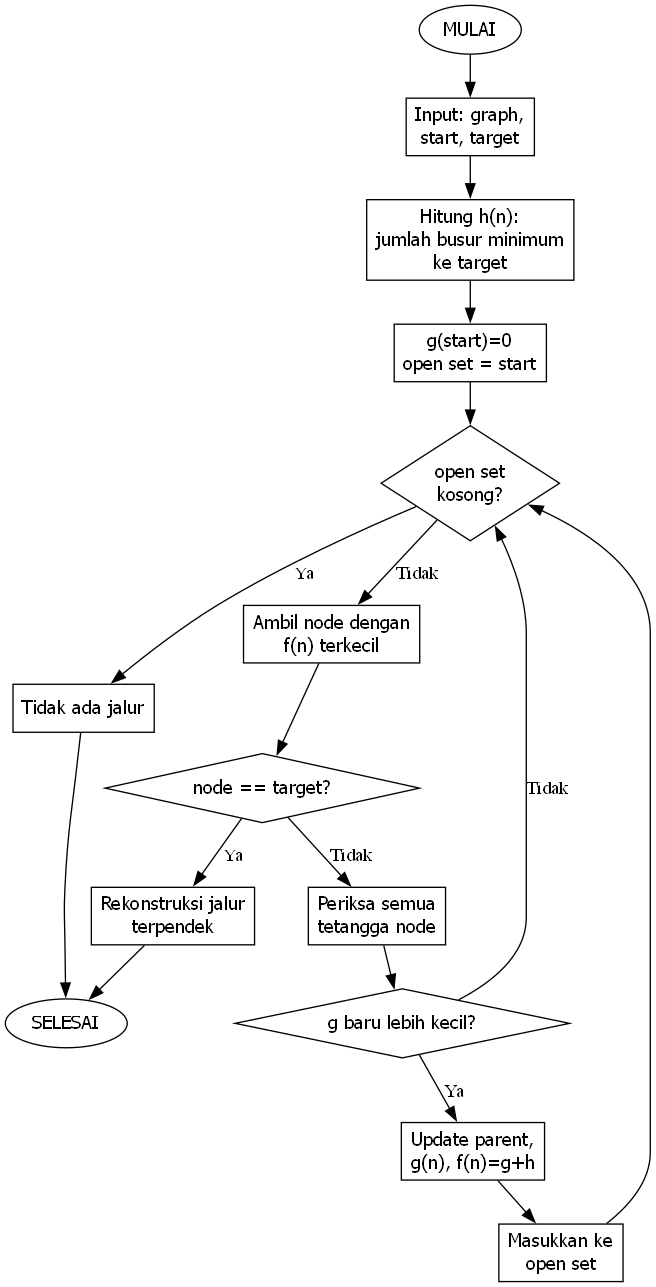
\includegraphics[width=0.55\textwidth]{figures/praktikum9/flowchart_astar.png}
    \caption{Flowchart Algoritma A*}
    \label{fig:praktikum9-flowchart-astar}
\end{figure}

\subsubsection*{Source Code Python}
Source code lengkap terdapat pada folder \texttt{src/praktikum9}. Bagian berikut hanya menampilkan inti program.

\textbf{1. Fungsi heuristik}
\begin{lstlisting}[basicstyle=\ttfamily\scriptsize, frame=single, backgroundcolor=\color{white}, numbers=none, keywordstyle=\color{black}, commentstyle=\color{black}, stringstyle=\color{black}, breaklines=true]
def compute_hop_heuristics(graph, target):
    heuristics = {node: inf for node in graph}
    heuristics[target] = 0
    queue = deque([target])

    while queue:
        node = queue.popleft()
        for neighbor, _ in graph[node]:
            if heuristics[neighbor] == inf:
                heuristics[neighbor] = heuristics[node] + 1
                queue.append(neighbor)

    return heuristics
\end{lstlisting}

\textbf{2. Fungsi utama A*}
\begin{lstlisting}[basicstyle=\ttfamily\scriptsize, frame=single, backgroundcolor=\color{white}, numbers=none, keywordstyle=\color{black}, commentstyle=\color{black}, stringstyle=\color{black}, breaklines=true]
def a_star(graph, start, target):
    heuristics = compute_hop_heuristics(graph, target)
    g_score = {node: inf for node in graph}
    parent = {node: None for node in graph}
    visited = set()
    queue = []

    g_score[start] = 0
    heappush(queue, (heuristics[start], 0, start))

    while queue:
        f_score, current_g, node = heappop(queue)
        if node in visited:
            continue
        visited.add(node)

        if node == target:
            return reconstruct_path(parent, target), g_score[target]

        for neighbor, edge_cost in graph[node]:
            tentative_g = g_score[node] + edge_cost
            if tentative_g < g_score[neighbor]:
                parent[neighbor] = node
                g_score[neighbor] = tentative_g
                new_f = tentative_g + heuristics[neighbor]
                heappush(queue, (new_f, tentative_g, neighbor))

    return [], inf
\end{lstlisting}

\textbf{3. Kode tester}
\begin{lstlisting}[basicstyle=\ttfamily\scriptsize, frame=single, backgroundcolor=\color{white}, numbers=none, keywordstyle=\color{black}, commentstyle=\color{black}, stringstyle=\color{black}, breaklines=true]
praktikum_edges = [
    (0, 1, 2), (0, 2, 4), (0, 4, 5), (1, 4, 1),
    (2, 3, 3), (3, 4, 3), (3, 5, 1), (4, 5, 2),
]

pretest_edges = [
    (0, 1, 3), (0, 2, 4), (0, 3, 5), (1, 3, 2),
    (2, 4, 4), (3, 4, 2), (4, 5, 1), (4, 6, 5),
    (5, 6, 3),
]

run_case("Graf praktikum Gambar 9.1", 6, praktikum_edges, 0, 5)
run_case("Graf pre/post test Gambar 9.2", 7, pretest_edges, 0, 6)
\end{lstlisting}

\subsubsection*{Analisis}
\textbf{Hasil graf praktikum:}
\begin{table}[H]
    \centering
    \caption{Hasil A* pada Graf Contoh Praktikum}
    \label{tab:praktikum9-hasil-praktikum}
    \begin{tabular}{ll}
    \toprule
    \textbf{Aspek} & \textbf{Hasil} \\ \midrule
    Start & 0 \\
    Target & 5 \\
    Jalur terpendek & [0, 1, 4, 5] \\
    Cost minimum & 5 \\
    Simpul diekspansi & 4 \\ \bottomrule
    \end{tabular}
\end{table}

\textbf{Post Test: A* pada Graf Gambar 9.2}
\begin{table}[H]
    \centering
    \caption{Validasi Hasil Program vs Manual pada Graf Gambar 9.2}
    \label{tab:praktikum9-validasi-posttest}
    \begin{tabular}{lll}
    \toprule
    \textbf{Sumber} & \textbf{Jalur Terpendek} & \textbf{Cost Minimum} \\ \midrule
    Manual Pre Test & 0--3--4--5--6 & 11 \\
    Program Python & [0, 3, 4, 5, 6] & 11 \\ \bottomrule
    \end{tabular}
\end{table}

\textbf{Kesimpulan:} Program menghasilkan jalur dan cost yang sama dengan analisis manual. Nilai $f(n)=g(n)+h(n)$ membantu memilih node yang paling menjanjikan.
